\documentclass[]{article}
\usepackage{packages}
\usepackage{listings}
\usepackage{booktabs}

\newcommand{\ve}[1]{\mathbf{#1}}

\begin{document}

\begin{center}
    \textbf{\LARGE FYS3500 MIDTERM HOME EXAM} \\
    \vspace{15pt}
    \textbf{Candidate number: } 15522 \\
    \vspace{15pt}
    \textit{In this assignement I mainly collaborated with candidate 155003. In addition I had some minor
    discussions with 15521, 15506, 15517 and I shared with them diagrams and figures.}
\end{center}

\vspace{30pt}

\section{Some shorter questions}
\subsection*{a}
This result can be explained by means of the nuclear shell model. According to this model each sub-level of the nucleus can be identified by 4 quantum numbers $\{n, j, l, m_l\}$. For fixed $\{n, j, l\}$ 
one has that the $2l+1$ sub-levels given by $m_l = -l, -l+1, \dots, l-1, l$ are degenerate and each of this sub-levels can contain two nucleons with different spin z-projrection ($m_s = \pm 1$). \\
At first one can notice that if one sub-shell is filled with two nucleons (of the same type) then the spin contibution of that sub-shell is 0. Having an even number of protons and neutrons means that 
they combine in couples in the sub-shell in a way such that the contribution to the spin of each sub-shell is 0. \\
For what concerns the parity, each particle in the nucleus gives a contribute of $(-1)^l$ (the intrinsic parity of the nucleons is $+1$) and the total parity is the product of single parities. 
The product of the parities of two protons (neutrons) in the same sub-shell is always $+1$ since they, in particular, share the same quantum number $l$. Hence it is legitimate to expect an even-even nucleus
to be in the state $0^+$.
\centerline{\textbf{Answer}: spin $0$, parity $+$}.

\section{Nuclear binding energy}
\subsection*{a}
The mass of the atom is given by
\begin{equation*}
    M(^{48}_{20}\text{Ca}^{28}) = Z(m_p + m_e) + (A-Z)m_n - \frac{B(A, Z)}{c^2}
    \label{eq:semi_empirical_mass_formula}
\end{equation*}
where $B$ indicates the binding energy, which in turns can be calculated via the semi-empirical formula (atomic units)
\begin{equation}
    B(A, Z)= a_v A - a_s A^{2/3} - a_c \frac{Z(Z-1)}{A^{1/3}} - a_{sym} \frac{(A - 2Z)^2}{A} + \delta (A, Z)
    \label{eq:semi_empirical_BE_formula}
\end{equation}
where 
\begin{equation*}
    \delta(A, Z) = 
    \begin{cases}
        \frac{a_P}{A^{1/2}} \qquad \text{if Z and N are even} \\
        0 \qquad \text{if A is odd} \\
        -\frac{a_P}{A^{1/2}} \qquad \text{if Z and N are odd} 
    \end{cases}
\end{equation*}
One can simply pop in the values of $A$ and $Z$ into the formula using the fitted coefficients (source Wikipedia) in units of $MeV/c^2$
\begin{equation*}
    a_v = 15.8 \qquad a_s = 18.3 \qquad a_c = 0.714 \qquad a_{sym} = 23.2 \qquad a_P = 12
\end{equation*}
and obtains $B(A, Z) = 412.84~MeV/c^2$. Hence, inserting the result into \ref{eq:semi_empirical_mass_formula} one obtains
\begin{equation*}
    M(^{48}\text{Ca}) \simeq 44670.64~MeV/c^2 \simeq 47.96~u
\end{equation*}
Thhe result is close to the experimental value ($47.952)$. One could justify eventual differences by observing that the SEMF is 
not a complete theoretical model, but rather a fit to experimental data of a model with some theoretical fundations. As such, it is reasonable that the model
can give an overall good description of the data but cannot perfectly describe each of them: this is especially the case of lighter atoms for which
the quantum shell structures of the nucleus should be taken into account.

\subsection*{b}
One can calculate the energy to remove a neutron as the difference in energy between the atom's state wth the neutron and without the neutron. The energy is the sum of
two terms, one that take accounts of the mass of the particles and it is simply the sum of all the masses. The second term, instead, is the binding energy. In the initial and final
state the mass energy contributions are the same (we are not making any particle disappear, we are just moving one away), hence the difference is only due to the binding energy contribution. One can
calculate this contribution as
\begin{equation*}
    B_{neutron} = B(A, Z) - B(A-1, Z)
\end{equation*}
and using expression \ref{eq:semi_empirical_BE_formula} with $A=44$ and $Z=20$ to calculate the two quantities one ends up with an estimation for the energy required to extract the neutron
\begin{equation*}
    B_{neutron} \approx 11.14~MeV/c^2
\end{equation*}

\subsection*{c}
One can search for the most stable atom with fixed $A$ searching for the minimum of the mass formula
\begin{equation*}
    M_A(Z) = Z(m_p + m_e) + (A-Z)m_n - B_A(Z)
\end{equation*}
Since one does not know if $Z$ is even or odd in advance, one can set the pairing term in the binding energy to $0$: this will lead to a non-integer $Z$ and 
the true minimum value will be either the closest greater or smaller integer (one has to check which of the two has minimum energy).
By direct calculation
\begin{equation*}
    0 = \frac{dM_A}{dZ} = m_p + m_e - m_n - \frac{a_c}{A^{1/3}} \left(A-2Z\right) + 4\frac{a_{symm}}{A} \left(A-2Z\right)
\end{equation*}
and rearranging terms
\begin{equation*}
    Z = \frac{m_n - (m_p + m_e) + 4a_{symm}A + a_c A^{2/3}}{2a_c A^{2/3} + 8a_{symm}} \approx 56.59 \qquad \longrightarrow \qquad Z = 56
\end{equation*}

\begin{figure}[h]
    \centering
    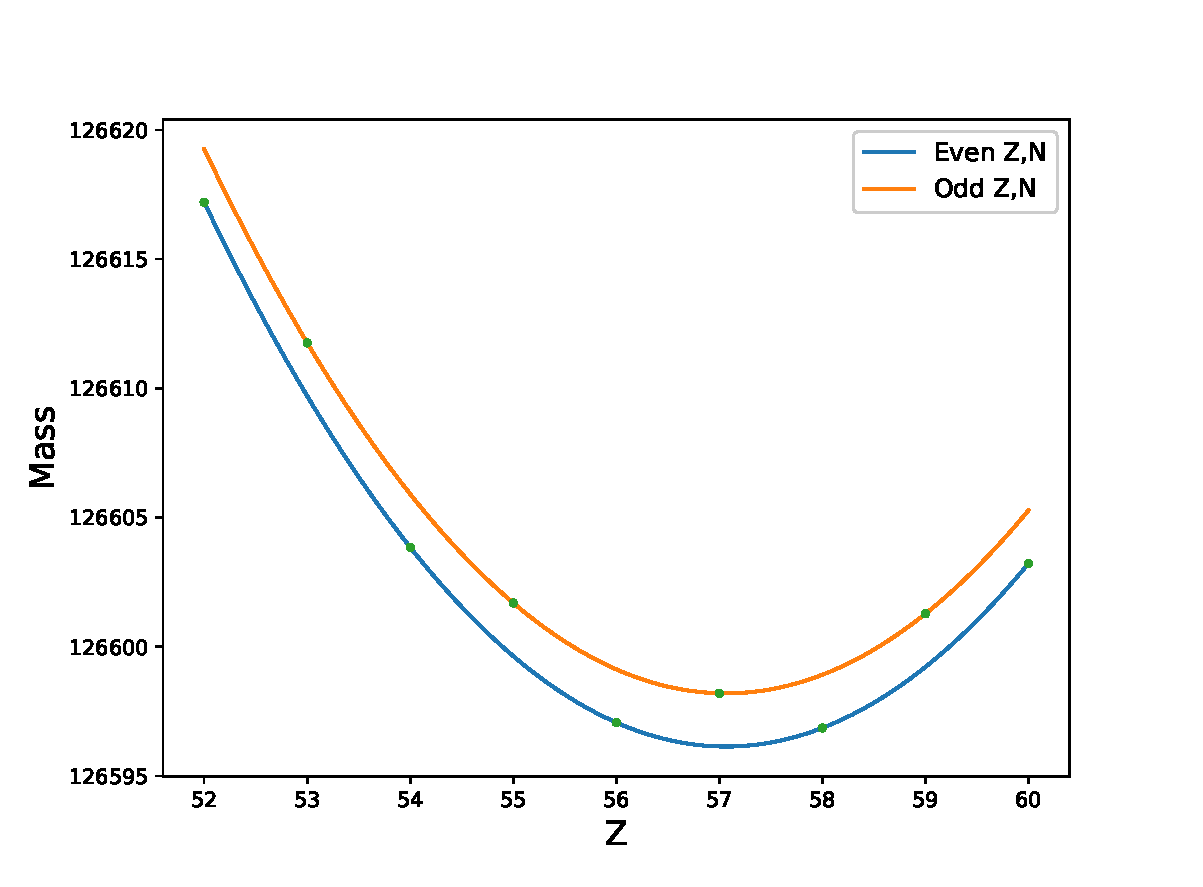
\includegraphics[scale=0.5]{ex2/evenA.eps}
    \caption{Even A}
\end{figure}
\begin{figure}[h]
    \centering
    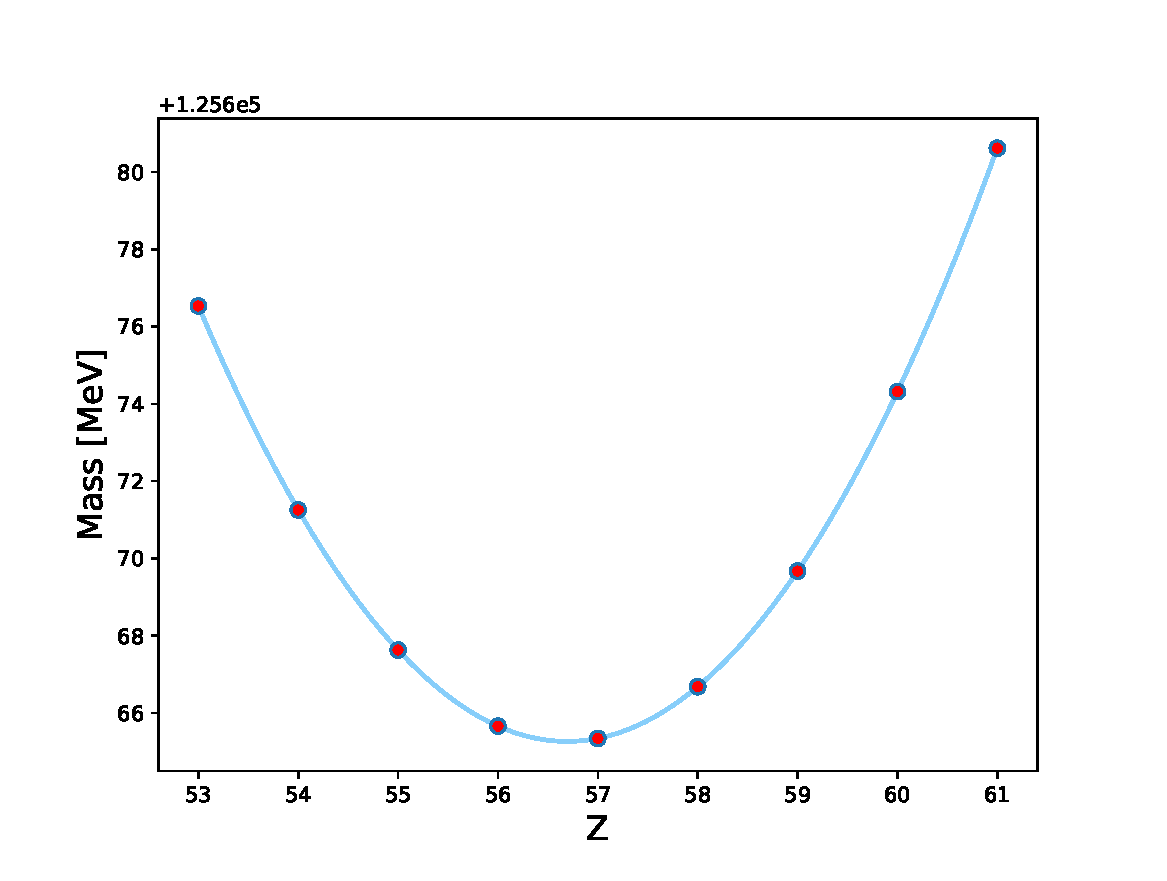
\includegraphics[scale=0.5]{ex2/oddA.eps}
    \caption{Odd A}
\end{figure}

\section{Higgs boson decay}
\subsection*{a}
In the resting frame of the Higgs boson the invariant mass is (atomic units)
\begin{equation}
    W = \sqrt{(\sum_i E_i)^2 - |\sum \ve{p}_i|^2} = E_H = m_H
    \label{eq:W_Higgs_frame}
\end{equation}
The invariant mass is a Lorent invariant, hence this quantity is the same that one observer would measure in the laboratory frame. 
More specifically, one can calculate $W$ after the process using the electrons data (laboratory frame)
\begin{equation*}
    W = \sqrt{(\sum_i E_i)^2 - |\sum \ve{p}_i|^2}
\end{equation*}
By equating this expression to \ref{eq:W_Higgs_frame} and inserting the given values together with the electrons mass one obtains
\begin{equation*}
    m_h \simeq 125.20~GeV/c^2
\end{equation*}

\subsubsection*{b}
In principle each pair of electron-positron can be generated by the $Z$ boson, in the sense that no rules would be violated. 
In other words there are $4$ different ways to combine the couples of electron-positron to the bosons
\begin{enumerate}
    \item $Z \rightarrow e^+_1 + e^-_1, \quad Z^* \rightarrow e^+_2 + e^-_2$
    \item $Z \rightarrow e^+_1 + e^-_2, \quad Z^* \rightarrow e^+_2 + e^-_1$ 
    \item $Z \rightarrow e^+_2 + e^-_1, \quad Z^* \rightarrow e^+_1 + e^-_2$
    \item $Z \rightarrow e^+_2 + e^-_2, \quad Z^* \rightarrow e^+_1 + e^-_1$
\end{enumerate}
One can now impose the conservation of the $4-$momentum in the bosons' decay and in particular, for the $Z$ boson, this means 
\begin{gather*}
    E_Z = \sqrt{m_Z^2 + p_Z^2} = E_{e^+} + E_{e^-} = \sqrt{m_{e^+}^2 + p_{e^+}^2} + \sqrt{m_{e^-}^2 + p_{e^-}^2} \\
\end{gather*}
and by rearrangin terms
\begin{gather*}
    p_Z^2 = (E_{e^+} + E_{e^-})^2 - m_Z^2
\end{gather*}
this equation gives the value of the momentum that the $Z$ boson must have in order to satisfy the conservation of the energy.
By explicit calculation for the $4$ cases, inserting the \href{https://en.wikipedia.org/wiki/W_and_Z_bosons}{Z boson mass}, one obtains 
\begin{enumerate}
    \item $p_Z^2 \simeq -2414~GeV/c$
    \item $p_Z^2 \simeq -7350~GeV/c$
    \item $p_Z^2 \simeq 744~GeV/c$
    \item $p_Z^2 \simeq  -5872~GeV/c$
\end{enumerate}
hence only in the third case the particle can be regarded as physical and not virtual.

\subsection*{c}
The invariant mass $W$ in the center of mass frame when the two $Z$ boson are generated is
\begin{equation*}
    W = \sqrt{E_Z + E_{Z^*}} = \sqrt{ \sqrt{p_Z^2 + m_Z^2} + \sqrt{p_Z^2 + m_{Z^*}^2}}
\end{equation*}
where I used the fact that $\ve p_Z = \ve p_{Z^*}$ by definition of center of mass. But for what told before $W=m_H$ hence, by squaring last equation 
\begin{equation*}
    m_H^2 = \sqrt{p_Z^2 + m_Z^2} + \sqrt{p_Z^2 + m_{Z^*}^2}
\end{equation*}
or
\begin{equation*}
    m_H^4 + p_Z^2 + m_Z^2 - 2m_H^2\sqrt{p_Z^2 + m_Z^2} = p_Z^2 + m_{Z^*}^2
\end{equation*}
which in turns leads to
\begin{equation*}
    p_Z^2 = \frac{m_H^2}{4} - m_Z^2
\end{equation*}
Hence the two energies are
\begin{equation*}
    E_Z = \sqrt{p_Z^2 + m_Z^2} = \frac{m_H}{2} \\
    E_{Z^*} = \sqrt{p_Z^2 + m_{Z^*}^2} = \frac{m_H}{2} = \sqrt{m_H^2 + m_{Z^*}^2 - m_Z^2}
\end{equation*}
and one can notice that if $m_Z = m_{Z^*}$ the energy of the Higgs boson $m_H$ is equally divided between the two Z bosons.
\subsection*{d}

\section{Lepton universality}
\subsection*{a}
Let us consider the two decays 
\begin{gather*}
    \tau^- \rightarrow \mu^- \, \bar\nu_{\mu} \, \nu_{\tau} \\
    \mu^- \rightarrow e^- \, \bar\nu_e \, \nu_{\mu}
\end{gather*}
represented by the two Feynman diagrams \\
\begin{figure}[hbtp]
    \centering
    \begin{minipage}{0.4\textwidth}
        \includegraphics[scale=0.6]{ex4/tau.png}
        \caption{Feynman diagram for the reaction $\tau^- \rightarrow \mu^- \, \bar\nu_{\mu} \, \nu_{\tau}$}
    \end{minipage}
    \hfill
    \begin{minipage}{0.4\textwidth}
        \includegraphics[scale=0.6]{ex4/mu.png}
        \caption{Feynman diagram for the reaction $\mu^- \rightarrow e^- \, \bar\nu_e \, \nu_{\mu}$}
    \end{minipage}
\end{figure}
The probability for a particle to get scattered by a certain potential is proportional to the squared of the so called \emph{amplitude} $\mathcal{M}$.
Assuming that the coupling constant $g^2$ of the Yukawa potential (atomic units)
\begin{equation*}
    V(r) = -\frac{g^2}{4\pi} \frac{e^{-r/R}}{r}
\end{equation*}
is small compared to $4\pi$ (this means that the potential can be considered as a perturbation to the free particle solution), then the amplitude $\mathcal{M}$ of the proces can be computed by means of the Born approximation
\begin{equation*}
    \mathcal{M}(\ve p) = \int V(\ve{r}) \, \exp(i\ve{r}\cdot\ve{r}) \, d^3\ve{r}
\end{equation*}
where $\ve{p} = \ve{p}_i - \ve{p}_f$ denotes the momentum difference between the initial and final state. By direct computation one can prove that 
\begin{equation}
    \mathcal{M}(\ve p) = \mathcal{M}(p^2) = - \frac{g^2}{p^2 + m_x^2}
    \label{eq:amplitude_born}
\end{equation}
where $m_x$ denotes the mass of the propagator. A multiplicative factor of $\sqrt{2}$ must be added if the spin interaction is taken into account. \\
In addition, the force carrier that governs the interaction is the $W$ boson, the mass of which is many times bigger than all the other involved masses. Hence a more suitable form of 
\ref{eq:amplitude_born} is 
\begin{equation*}
    \mathcal{M}(\ve p) = \mathcal{M}(p^2) = - \sqrt{2} \, \frac{g^2}{m_x^2} \approx 1.166 \cdot 10^{-5}~(GeV)^{-2} \equiv G_F
\end{equation*}
and $G_F$ is the Fermi coupling constant.
This results is known as \emph{leptons universality} and states that the amplitude of a lepton's decay process is a constant that does not depend on the chosen lepton. \\
At this point one can introduce the decay rate $\Gamma$ which is proportional to the probability of the process to occur
\begin{equation*}
    \Gamma \approx K M^2 A
\end{equation*}
where $A$ is a constant whose units are those of an energy to the fifth power, because $[M^2] = (GeV)^{-4}$. Since we expect the decay rate 
to depend on the generating particle, a reasonable choice for $A$ is $A=m_i^5$ where indeed $m_i$ denotes the mass of the generating particle. Hence
\begin{equation*}
    \Gamma \approx - \sqrt{2} K \, \frac{g^2}{m_x^2}m_i^5
\end{equation*}
Applying it to the particular case of the two given processes one obtains
\begin{equation}
    \frac{\Gamma\left(\tau^- \rightarrow \mu^- \, \bar\nu_{\mu} \, \nu_{\tau}\right)}{\Gamma\left( \mu^- \rightarrow e^- \, \bar\nu_e \, \nu_{\mu}\right)}
    \approx \left(\frac{m_{\tau}}{m_{\mu}}\right)^5 \approx 1.34 \cdot 10^6
    \label{eq:decay_widths_ratios}
\end{equation}

\subsection*{b}
The two relevant experimental quantities are the lifetime of the particles $\tau$ and the brancing ratios of the reactions. Let us define
$\Gamma_{\tau} \equiv \Gamma(\tau \to X \nu_{\tau})$ and $\Gamma_{\mu} \equiv \Gamma(\tau \to Y \nu_{\mu})$. Equation \ref{eq:decay_widths_ratios} 
can be rewritten as 
\begin{equation*}
    \frac{\Gamma\left(\tau^- \rightarrow \mu^- \, \bar\nu_{\mu} \, \nu_{\tau}\right)}{\Gamma\left( \mu^- \rightarrow e^- \, \bar\nu_e \, \nu_{\mu}\right)} =
    \frac{\Gamma\left(\tau^- \rightarrow \mu^- \, \bar\nu_{\mu} \, \nu_{\tau}\right)}{\Gamma_{\tau}} \
    \frac{\Gamma_\mu}{\Gamma\left( \mu^- \rightarrow e^- \, \bar\nu_e \, \nu_{\mu}\right)} \
    \frac{\Gamma_{\tau}}{\Gamma_{\mu}} = 
    \frac{B\left(\tau^- \rightarrow \mu^- \, \bar\nu_{\mu} \, \nu_{\tau}\right)}{B\left( \mu^- \rightarrow e^- \, \bar\nu_e \, \nu_{\mu}\right)} \ 
    \frac{\tau_{\mu}}{\tau_{\tau}}
\end{equation*}
which is a more relevant form for the experimental quantities.

\section{Quantum numbers}
\subsection*{a} 
\vspace{10pt}
\emph{Parity} \\
\vspace{10pt} \\
Let us consider a wavefunction $\psi(\ve r)$. One can define the parity operator $\hat P$ as an operator such that 
\begin{equation*}
    \hat P \, \psi(\ve r) = \psi(-\ve r)
\end{equation*}
Since
\begin{equation}
    \hat P^2 \, \psi(\ve r) = \hat P \, \psi(-\ve r) = \psi(\ve r)
    \label{eq:eigenvalue_equation_parity}
\end{equation}
the eigenvalues of the parity operator are $\pm 1$ and the corresponding eigenfunctions are the odd (eigenvalue $-1$) and even (eigenvalue $+1$) wavefunctions. If the wavefunction
describes the state of particle, and the state is an eigenstate of the parity operator, the corresponding eigenvalue is also said to be the (intrinsic) parity of the particle. \\
Let us consider a system of two particles $A+B$ described by a wavefunction $\psi_{AB}(\ve{r}_A, \ve{r}_B)$. It can be proven that the parity of the system is given by 
\begin{equation*}
    \hat P \psi_{AB} = \pi_A \pi_B (-1)^l \psi_{AB}
\end{equation*}
where $l$ denotes the orbital angular momentum quantum number of the relative motion. Hence in a reaction of the type $A+B \rightarrow C+D$ described by a hamiltonian $\hat H$ that commutes with parity,
parity is conserved or, in other words
\begin{equation*}
    \pi_A \pi_B (-1)^{l_{AB}} = \pi_C \pi_D (-1)^{l_{CD}} 
\end{equation*}
This, for example, is not the case of the weak interaction where, in general, the hamiltonian operator does not commute with the parity operator. \\
\vspace{10pt} \\
\emph{Charge conjugation} 
\vspace{10pt} 

\subsection*{c}
$^{15}$N atom has 7 protons and 8 neutrons. Since the neutrons (in the ground state) are all coupled (each sub-shell admits two nucleons) they do not contribute to  the spin of the nucleus and the parity contribution is $+1$. Instead the protons configuration
of the $^{15}$N atom in the ground state is $(1s)^2 \, (1p_{3/2})^2 \, (1p_{1/2})^1$: only the last proton contributes to the interested quantities. Since the orbital $p$ represents the quantum number $l=1$ the parity of the the nucleus is the product of the neutrons 
an protons contribution, that is $(+1) \cdot (-1)^1 = -1$. The spin is then $1/2$. \\
There are three possible alternatives for the first excited state, all of which consists in moving a proton or a neutron to another level starting from the ground state configuration.
\begin{enumerate}
    \item Move the $1p_{1/2}$ proton to the $1d_{5/2}$ level \\ $\quad \longrightarrow \quad$ the new proton configuration is $(1s)^2 \, (1p_{3/2})^2 \, (1p_{1/2})^{-2} \, (1d_{5/2})^1$ and the spin-parity is $1/2^+$.
    \item Move the $1p_{3/2}$ proton to the $1d_{5/2}$ level \\ $\quad \longrightarrow \quad$ the new proton configuration is $(1s)^2 \, (1p_{3/2})^{-1} \, (1p_{1/2})^2$ and the spin-parity is $3/2^-$.
    \item Move the $1p_{1/2}$ neutron to the $1d_{5/2}$ level \\ $\quad \longrightarrow \quad $ the new neutorn configuration is $(1s)^2 \, (1p_{3/2})^2 \, (1p_{1/2})^{-1} \, (1d_{5/2})^1$. The parity here is non-trivial because of the angular momemnta addition rules.
\end{enumerate}
By looking at the suggested table, one can notice that the first excited state is described by configuration $3$, the second by configuration $1$ and the third excited state is described by configuration $2$.


\begin{figure}
    \centering
    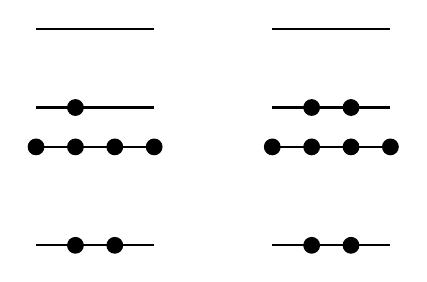
\begin{tikzpicture}
        
        % Protons
        \foreach \x in {0, 3}{
            \foreach \y in {0, 1.25, 1.75, 2.75}{
                \draw [thick] (\x, \y) -- ++(1.5, 0);
            }
            \node[draw, circle, inner sep=2pt, fill] at (\x+0.5, 0){};
            \node[draw, circle, inner sep=2pt, fill] at (\x+1, 0)(1.5,0){};
            \node[draw, circle, inner sep=2pt, fill] at (\x, 1.25){};
            \node[draw, circle, inner sep=2pt, fill] at (\x+0.5, 1.25){};
            \node[draw, circle, inner sep=2pt, fill] at (\x+1.5, 1.25){};
            \node[draw, circle, inner sep=2pt, fill] at (\x+1, 1.25){};
            \node[draw, circle, inner sep=2pt, fill] at (\x+0.5, 1.75){};
        }
        \node[draw, circle, inner sep=2pt, fill] at (4, 1.75){};
    \end{tikzpicture}
    \caption{nothing}
    \label{fig:nitrogen_nucleons_ground_state}
\end{figure}


\begin{figure}
    \centering
    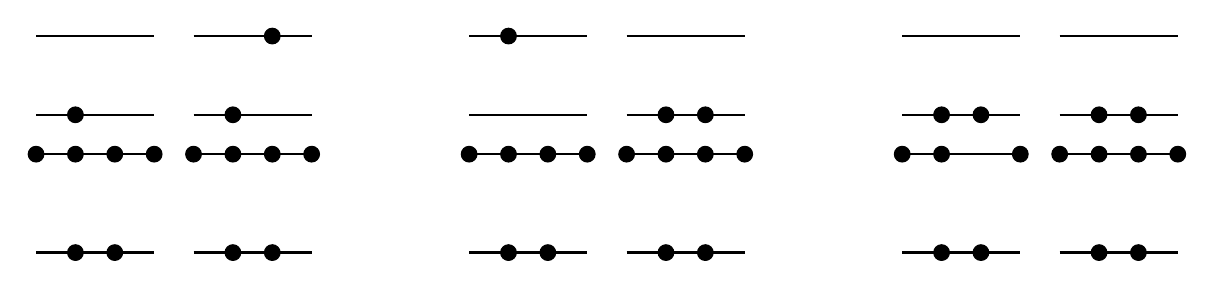
\begin{tikzpicture}

        % Protons
        \foreach \x in {0.5, 6, 11.5}{
            \foreach \y in {0, 1.25, 1.75, 2.75}{
                \draw [thick] (\x, \y) -- ++(1.5, 0);
            }
            \node[draw, circle, inner sep=2pt, fill] at (\x+0.5, 0){};
            \node[draw, circle, inner sep=2pt, fill] at (\x+1, 0)(1.5,0){};
            \node[draw, circle, inner sep=2pt, fill] at (\x, 1.25){};
            \node[draw, circle, inner sep=2pt, fill] at (\x+0.5, 1.25){};
            \node[draw, circle, inner sep=2pt, fill] at (\x+1.5, 1.25){};
        }
        \node[draw, circle, inner sep=2pt, fill] at (1, 1.75){};
        \node[draw, circle, inner sep=2pt, fill] at (6.5, 2.75){};
        \node[draw, circle, inner sep=2pt, fill] at (12, 1.75){};
        \node[draw, circle, inner sep=2pt, fill] at (3.5, 2.75){};
        \node[draw, circle, inner sep=2pt, fill] at (9, 1.75){};
        \node[draw, circle, inner sep=2pt, fill] at (14.5, 1.75){};
        \node[draw, circle, inner sep=2pt, fill] at (1.5, 1.25){};
        \node[draw, circle, inner sep=2pt, fill] at (7, 1.25){};
        \node[draw, circle, inner sep=2pt, fill] at (12.5, 1.75){};

        % Neutrons
        \foreach \x in {2.5, 8, 13.5}{
            \foreach \y in {0, 1.25, 1.75, 2.75}{
                \draw [thick] (\x, \y) -- ++(1.5, 0);
            }
            \node[draw, circle, inner sep=2pt, fill] at (\x+0.5, 0){};
            \node[draw, circle, inner sep=2pt, fill] at (\x+1, 0)(1.5,0){};
            \node[draw, circle, inner sep=2pt, fill] at (\x, 1.25){};
            \node[draw, circle, inner sep=2pt, fill] at (\x+0.5, 1.25){};
            \node[draw, circle, inner sep=2pt, fill] at (\x+1, 1.25){};
            \node[draw, circle, inner sep=2pt, fill] at (\x+1.5, 1.25){};
            \node[draw, circle, inner sep=2pt, fill] at (\x+0.5, 1.75){};
        }

    \end{tikzpicture}
    \caption{nothing}
    \label{fig:nitrogen_nucleons_excited_states}
\end{figure}

\section{Allowed, suppressed and forbidden processes}
I use the definition of decay stated \href{https://en.wikipedia.org/wiki/Particle_decay}{here}. \\
I do not follow the order of the questions as given, but everything is reported here.
\begin{table}[htbp]
    \centering
    \begin{tabular}{cccccc}
        \toprule
            Process & Type & Interaction & Allowed & Suppressed & Reason not allowed \\
        \midrule 
            $1$ & decay & electroweak & yes & no & \\
            $2$ & & & no & & charge \\
            $3$ & decay & electroweak & yes & yes & \\
            $4$ & decay & weak & yes & no & \\
            $5$ & decay & strong & yes & no & \\
            $6$ & reaction & electroweak + strong & yes & no & \\
            $7$ & decay & weak & yes & no & \\
            $8$ & & & no & & lepton number \\
        \bottomrule
    \end{tabular}
\end{table}

\begin{figure}[hbtp]
    \centering
    \includegraphics[scale=0.05]{Feynman/cc-_cc-01.jpg}
    \includegraphics[scale=0.2]{Feynman/decaycircular.jpg}
    \includegraphics[scale=0.05]{Feynman/Delta+-01.jpg}
    \includegraphics[scale=0.05]{Feynman/eeqq-01.jpg}
    \includegraphics[scale=0.05]{Feynman/lambda0-01.jpg}
    \includegraphics[scale=0.2]{Feynman/neutrinoless.jpg}
    \includegraphics[scale=0.05]{Feynman/worldwouldbeboring-01.jpg}
\end{figure}

\begin{table}[hbtp]
    \centering 
    \begin{tabular}{cccc}
        \toprule
            Process & Interaction & Typical Interaction time & Lifetime \\
        \midrule
            1 & electromagnetic & $10^{-14} \sim 10^{-20}$ & \\
            3 & weak & $10^{-8} \sim 10^{-13}$ & $10^{-12}$ \\
            4 & weak & $10^{-8} \sim 10^{-13}$ & $10^{-10}$ \\
            5 & strong & $<10^{-22}$ & $10^{-24}$ \\
        \bottomrule
    \end{tabular}
\end{table}

Process 3 is not the most common decay for the bottom quark, hence extremely rare and suppressed. \\
Processes 7 and 8 differ by the presence of 2 antineutrinos. The process 8, namely the neutrinoless double beta decay,
is not allowed according to the Standard model because it violates the lepton number conservation. The observation of such 
decay would indeed confirm the Majorana nature of the neutrinos and the lepton number conservation rule would be violated. \\
When neutron deacys into 2 protons and 2 electrons without the neutrino, the energy is equally splitted to the generated particles 
according to their masses. On the opposite, when the antineutrinos are produced, part of the energy would be transferred to them,
but the portion is not fixed, hence it would produce a continuous energy spectrum.



\section{Radioactive decay}
\begin{figure}[htbp]
    \centering
    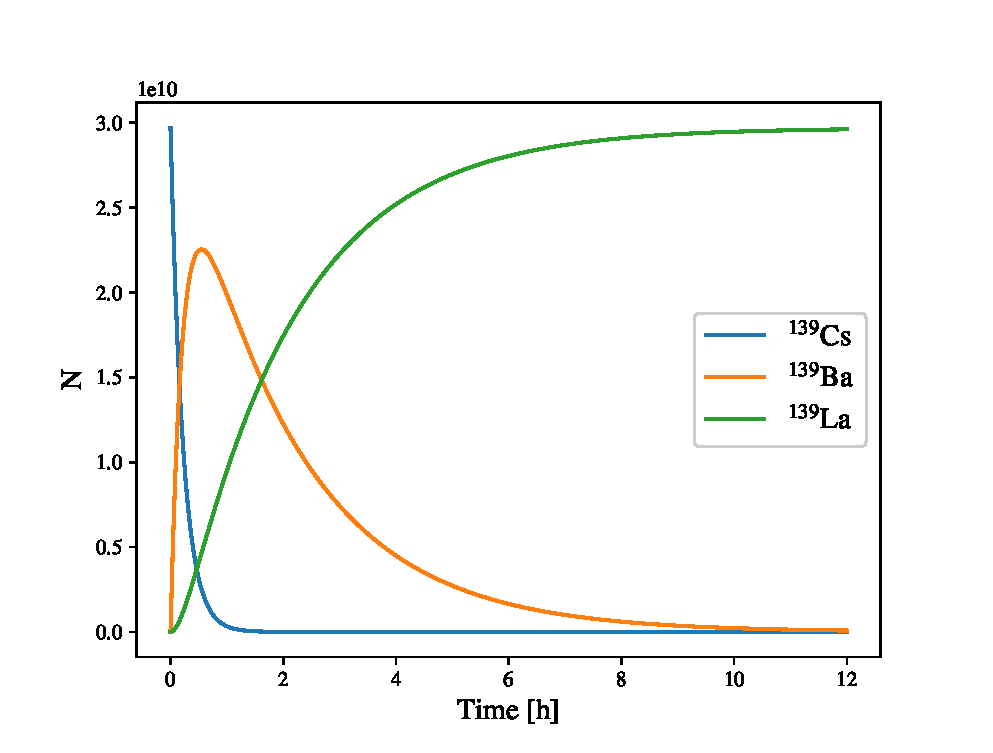
\includegraphics[scale=0.8]{ex7/decay.eps}
    \caption{Radioactive decay chain}
    \label{fig:decay_chain}
\end{figure}

\lstinputlisting[language=python, showstringspaces=false]{ex7/ex7.py}

\section{Code for exercise 1}
\lstinputlisting[language=python, showstringspaces=false]{ex1/nucleons.py}

\section{Code for exercise 2}
\lstinputlisting[language=python, showstringspaces=false]{ex2/ex2.py}

\section{Code for exercise 3}
\lstinputlisting[language=python, showstringspaces=false]{ex3/higgs.py}

\section{Code for exercise 7}
\lstinputlisting[language=python, showstringspaces=false]{ex7/ex7.py}

\end{document}